\begin{figure}[t]\centering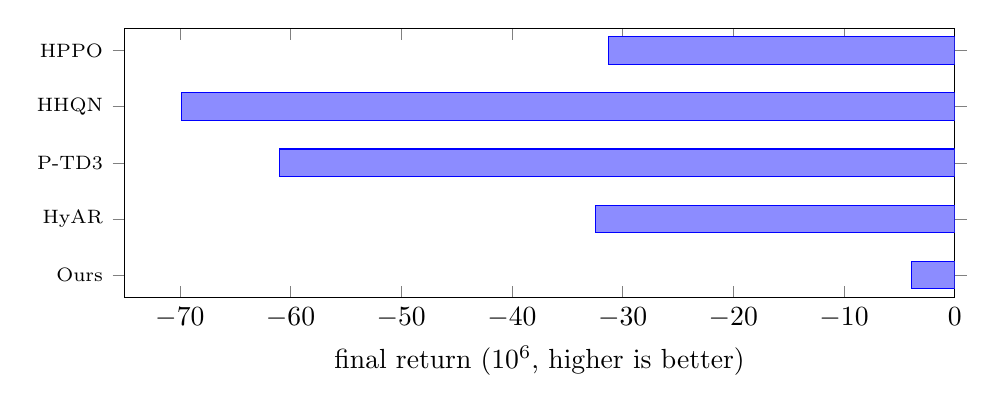
\begin{tikzpicture}\begin{axis}[width=\linewidth,height=5cm,xbar,xmin=-75,xmax=0,xlabel={final return ($10^6$, higher is better)},symbolic y coords={Ours,HyAR,P-TD3,HHQN,HPPO},ytick=data,yticklabel style={font=\scriptsize}]
\addplot+[fill=blue!45] coordinates {(-3.927,Ours)(-32.471,HyAR)(-61.003,P-TD3)(-69.854,HHQN)(-31.263,HPPO)};
\end{axis}\end{tikzpicture}\caption{Cogen-BC sealed final return. The environment is the action-restricted Cogen-BC variant; values closer to zero are higher.}\label{fig:cogenret}\end{figure}
